\documentclass[review,letterpaper,11pt]{elsarticle}

\biboptions{numbers,sort&compress}
\usepackage{amsmath,amssymb,amsfonts,amsthm}
\usepackage{graphicx}
\usepackage{textcomp}
\usepackage{xcolor, color}
\usepackage{hyperref}       % hyperlinks
\usepackage{url}            % simple URL typesetting
\usepackage{bm}
\usepackage{booktabs}       % professional-quality tables
\usepackage{nicefrac}       % compact symbols for 1/2, etc.
\usepackage{microtype}      % microtypography
\usepackage{psfrag}
\usepackage{lipsum,siunitx}
\usepackage{epstopdf}

\newcommand*{\horzbar}{\rule[.5ex]{2.5ex}{0.5pt}}
\newcolumntype{T}[1]{S[table-format=#1,group-digits=false]}

%\usepackage[section]{placeins}
% Li's TeX stuff
% \usepackage{enumerate}
% \usepackage{environ} %% New way for defining environments.
% \usepackage{hhline}

\begin{document}

\begin{frontmatter}

\title{Driving Markov Chains to Desired Equilibria}

\author[ucm,utah]{Harish~S. Bhat\corref{cor}}
\ead{hbhat@math.utah.edu}

\author[ucm]{Li-Hsuan Huang}
\ead{lhuang33@ucmerced.edu}

\author[nw]{Sebastian Rodriguez}
\ead{SebastianRodriguez2022@u.northwestern.edu}

\cortext[cor]{Corresponding author}

\address[ucm]{Applied Mathematics Unit, University of California, Merced, 5200 North Lake Rd, Merced, CA 95343 USA}
\address[utah]{Department of Mathematics, University of Utah, 155 S 1400 E RM 233, Salt Lake City, UT 84112 USA}
\address[nw]{Department of Statistics, Northwestern University, 2006 Sheridan Rd, Evanston, IL 60208 USA}

\begin{abstract}
We address the issue of statistically estimated, absorbing Markov chains whose equilibria differ signifcantly from observations of how much time is spent in each state.  We propose an optimization method that yields a sparse perturbation of the original Markov chain; this perturbation is constrained to achieve a desired equilibrium, while maintaining the properties of a valid Markov chain.  We establish this formulation for both discrete- and continuous-time Markov chains and translate these formulations into linear programming problems that can be solved efficiently and accurately.  We apply this optimization procedure to simulated and real data, demonstrating its competitive performance. In particular, we develop improved models to predict the time played by each 5-person unit for each NBA team.
\end{abstract}

\begin{keyword}
Markov chains, estimation, absorbing state, optimization
\end{keyword}

\end{frontmatter}

\section{Introduction}
\label{sect:intro}

We study the problem of estimating Markov chain models for discrete-state systems.  Suppose we observe such a system continuously in time as it transitions from one state to the next.  Further suppose that there exists a set of one or more states (say, $S$) from which the system never transitions to another state.  Maximum likelihood estimation will then yield a Markov chain model in which the states in $S$ are absorbing.  Consequently, the equilibrium or stationary distribution associated with the Markov chain will be supported only on $S$.  The estimated model will assign a probability of zero to the long-term probability of spending time in states other than $S$.  For several systems of interest, this will destroy the predictive power of the estimated model.

Our motivating example arises in the area of basketball analytics.  To model substitutions and minutes played by each player for real NBA (National Basketball Association) games, we have built continuous-time Markov chain models.  For a given team, each state corresponds to a distinct unit of five players on the court.  Transitions from one state to another correspond to the substitution of one or more players.  Given a time-stamped, play-by-play transcript of a game, we know exactly how long each five-person unit played on the court and exactly when substitutions occurred---in this sense, the system is observed continuously in time.  In many regular-season NBA games, when one team is ahead by a large margin towards the end of the game, there is a high probability that one team (or both teams) will substitute in rookies or non-starting players.  Hence it is likely that the last observed state (say, $\sigma$) of the system is a state that has been reached for the first time in the game (and possibly for the first time in the entire season).  As described above, in the estimated model, $\sigma$ will then be an absorbing state.  The equilibrium distribution for the estimated model will then have nothing to do with the empirical fraction of time actually spent in each state.

The main contribution of this paper is a a pair of algorithms for removing absorbing states from both continuous-time Markov chain (CTMC) and discrete-time Markov chain (DTMC) models.  In both the CTMC and DTMC cases, the model is specified by an $M \times M$ matrix $\widehat{p}$, where $M$ is the number of states.  Starting from the maximum likelihood estimate (MLE) of $\widehat{p}$, we ask: what is the most sparse perturbation $\varepsilon$ that yields an absorbing-state-free Markov chain $\widehat{p} + \varepsilon$ whose equilibrium vector exactly matches the observed fraction of time spent in each state?  We formulate this question as an optimization problem and show how to solve it efficiently using linear programming.

While we have not found published work that solves the problems outlined above, we can certainly identify subsets of the literature that help contextualize the present work.  Perhaps the most relevant subset is that dealing with inverse eigenvector problems for nonnegative matrices---see \cite{chu1998numerical,chu2005inverse,bai2012nonnegative}.  Here we find techniques to construct nonnegative matrices with prescribed eigenvalues and eigenvectors.  Once such a nonnegative matrix has been constructed, it can be transformed into a stochastic matrix, i.e., a transition matrix for a DTMC.  It is entirely possible to use these methods to construct a DTMC whose equilibrium vector matches data, i.e., matches the empirical fraction of time spent in each state.  Special algorithms to deal with this particular case of the inverse eigenvector problem have been developed \cite{KTVVwsdm15, maystre2015fast}.  However, there is no link between these techniques and short-term trends in the data---for each $i \neq j$, the $(i,j)$ entry of the resulting stochastic matrix does not necessarily have anything to do with the empirical frequency of transitions from state $i$ to state $j$.  In contrast, our method \emph{constrains} the estimated model to be close to these frequencies, i.e., the MLE estimates $\widehat{p}_{i,j}$.

Note that inverse eigenvector methods can be used to construct Markov Chain Monte Carlo (MCMC) methods with optimal properties \cite{Chu2015}.  We plan to explore in future work whether the methods from the present paper can be used in the MCMC context.  Note also that the inverse eigenvector problem---in which a desired eigenvalue-eigenvector pair is prescribed---is different from inverse problems for eigenvalues only \cite{Laurie1991, chen2011isospectral, yao2016riemannian}.  

The next subset of papers deals with PageRank, a fundamental algorithm used to rank web pages \cite{Langville2006}.  Consider a collection $\mathcal{C}$ of $M$ interlinked web pages and treat each web page as a Markov chain state.  If there are $n$ links on a particular web page, we assign a probability of $1/n$ to transition from that particular web page to each of the linked pages.  This gives us a Markov chain corresponding to a random walk on the graph corresponding to $\mathcal{C}$.  Also consider the $M \times M$ stochastic matrix in which each entry is $1/M$---this corresponds to a Markov chain in which all states communicate uniformly with all other states.  The PageRank DTMC model consists of a linear combination of the random walk and uniform transition matrices; if the weights in the linear combination sum to $1$, the resulting matrix is itself a valid Markov chain.  The equilibrium vector of the PageRank DTMC model can then be used to rank web pages.

There has been significant development in estimating/analyzing how this equilibrium vector changes when links between web pages are changed \cite{NZJijcai01, langville2006updating, Chartier2011}, and also in optimizing the PageRank vector according to various criteria and methods \cite{fercoq2013ergodic, fercoq2014perron, csaji2014pagerank}.  Given a desired PageRank equilibrium vector $w$ and a PageRank DTMC model $\widehat{p}$ that has already been estimated, our algorithm computes the most sparse perturbation $\varepsilon$ that yields a DTMC model $\widehat{p} + \varepsilon$ with equilibrium $w$.  Suppose we treat the web graph as weighted, as in weighted PageRank \cite{Gleich2015} or certain link recommendation models \cite{backstrom2011supervised}.  Then the $\varepsilon$ developed by our algorithm tells us how to adjust weights to achieve a desired ranking of pages.

Finally, we should mention that the problem of estimating CTMC models from \emph{temporally discrete} observations is entirely different from the problem considered here.  If we only observe the CTMC process at discrete times, then we do not necessarily know that those times correspond to transitions, nor can we rule out transitions occurring at times in between the times at which we have data.  This leads to a more complex estimation problem that has attracted much recent interest---see \cite{Schutte2007, Rao2013, Hajiaghayi2014, Crawford2014}.

\section{Background}
\label{sect:background}
For the purposes of this paper, we describe Markov chains via the methods we use to generate sample trajectories.  For more mathematical definitions, consult \cite{Lawler}.

A DTMC with $M$ states is determined by an $M \times M$ transition matrix $p$.  
Suppose the DTMC is currently in state $i$.  We examine $p_i$, row $i$ of the matrix $p$.  To be a valid transition matrix, each $p_i$ must be a probability mass function over the state space.  To generate the next sample in the trajectory, we sample from the distribution $p_i$; this yields a state $i' \in \{1, 2,  \ldots, M\}$.

To continue, we repeat the above procedure, starting in state $i'$.  In this way, we can generate trajectories of arbitrary length, consisting of sequences of states.

A CTMC with $M$ states is determined by an $M \times M$ transition rate matrix $p$.  Suppose the CTMC is currently in state $i$.  We examine $p_i$, row $i$ of the matrix $p$.  The entries of $p_i$ off the diagonal must be nonnegative---we treat these entries as parameters of $M-1$ independent, exponentially distributed random variables.  We draw one sample from each exponential random variable.  The minimum of these samples represents how long we spend in state $i$ before transitioning.  The argmin of these samples represents the new state $i'$ to which we transition.

To continue, we repeat the above procedure, starting in state $i'$.  In this way, we can generate trajectories of arbitrary length, consisting of sequences of states and corresponding transition times.

\section{Mathematical Methods}
\label{sect:method}

\subsection{DTMC Optimization Problem and Solution} 
Let us first consider the problem for DTMC models.  Suppose we have an $M \times M$ transition matrix $\widehat{p}$, estimated using MLE, that has absorbing states.  We seek a perturbation $\varepsilon$ such that $\widehat{p} + \varepsilon$ has no absorbing states.  We still want $\widehat{p} + \varepsilon$ to be a valid Markov transition matrix, so we require that
\begin{equation}
\label{eqn:newdtmcequality1}
\sum_{j} ( \widehat{p}_{i,j}+\varepsilon_{i,j} )= 1.
\end{equation}
Of course, $\sum_j \widehat{p}_{i,j} = 1$ already, implying
\begin{equation}
\label{eqn:newdtmcequality2}
\sum_{j} \varepsilon_{i,j} = 0.
\end{equation}
Because of this constraint, we only need to solve for the off-diagonal part of $\varepsilon$, a total of $M^2 - M$ unknowns.  We set
\begin{equation}
\label{eqn:newdtmcequality3}
\varepsilon_{i,i} = -\sum_{j \neq i} \varepsilon_{i,j}.
\end{equation}
Assume that $w$ is a desired equilibrium vector.  This yields an additional constraint:
$$
w^T (\widehat{p} + \varepsilon) = w^T.
$$
In coordinates, this reduces to
$$
\sum_{i \neq j} w_i \varepsilon_{i,j} - \sum_{i \neq j} w_j \varepsilon_{j,i} = w_j - \sum_i w_i \widehat{p}_{i,j}.
$$
The entries of the perturbed matrix must also be valid probabilities:
$$
0 \leq \widehat{p}_{i,j} + \varepsilon_{i,j} \leq 1
$$
for all $i$ and all $j$.  For $i \neq j$, we can enforce this constraint verbatim.  For $i = j$, we use (\ref{eqn:newdtmcequality3}) to rewrite the constraint as:
$$
0 \leq \widehat{p}_{i,i} - \sum_{j \neq i} \varepsilon_{i,j} \leq 1.
$$
For each $i$, we enforce the lower bound of $0$:
$$
\sum_{j \neq i} \varepsilon_{i,j} \leq \widehat{p}_{i,i}.
$$
However, for the upper bound, we replace $1$ by $w_i$ and require, for each $i$,
\begin{equation}
\label{eqn:DTMCdiagconstr}
-\sum_{j \neq i} \varepsilon_{i,j} + \widehat{p}_{i,i} \leq w_i.
\end{equation}
In this paper, we will take $w$ to be a candidate equilibrium distribution with no absorbing states, i.e., $0 < w_i < 1$ for each $i$.  Hence (\ref{eqn:DTMCdiagconstr}) and (\ref{eqn:newdtmcequality3}) guarantee that $\varepsilon_{ii} + \widehat{p}_{ii} \leq \max_i w_i < 1$.  In short, the diagonal entries of the perturbed transition matrix $\widehat{p} + \varepsilon$ are bounded away from $1$, implying that the perturbed system cannot have any absorbing states.

We also enforce (\ref{eqn:DTMCdiagconstr}) because we know that the Markov transition matrix given by
\begin{equation}
\label{eqn:dtmcguarantee}
\widehat{p} + \varepsilon = 
\begin{bmatrix} \horzbar w \horzbar \\
\horzbar w \horzbar \\
\vdots \\
\horzbar w \horzbar
\end{bmatrix}
\end{equation}
automatically has equilibrium distribution $w$.  Hence we know there exists at least one feasible solution where the diagonal elements satisfy $\widehat{p}_{ii} + \varepsilon_{ii} = w_i$.

We now consider the choice of objective function.  A natural first choice might be the sum of the squares of the off-diagonal elements of $\varepsilon$, essentially a form of the $2$-norm.  This objective function does not promote sparsity.  It is likely that the resulting solution will cause each MLE $\widehat{p}_{i,j}$ to be perturbed.  We view this as undesirable.

Instead, we would like to find a new transition matrix $\widehat{p} + \varepsilon$ that retains as many of the original MLE entries $\widehat{p}$ as possible.  In other words, we want to maximize the number of zero entries of $\varepsilon$.  Consequently, we set our objective function equal to the sparsity-promoting $1$-norm of the off-diagonal elements of $\varepsilon$:
\begin{equation*}
J(\varepsilon) = \sum_{i,j : i \neq j} |\varepsilon_{i,j}|.
\end{equation*}
Putting the objective and constraints together, we are led to the following optimization problem:
\begin{equation}
\label{eqn:dtmcopt1}
\begin{aligned}
& \underset{\varepsilon}{\text{min}}
& & J(\varepsilon) \\
& \text{s.t.}
& & 0 \leq \widehat{p}_{i,j} + \varepsilon_{i,j} \leq 1, \; \forall i \neq j \\
&&& 0 \leq -\sum_{j \neq i} \varepsilon_{i,j} + \widehat{p}_{i,i} \leq w_i, \; \forall i \\
&&& \sum_{i \neq j} w_i \varepsilon_{i,j} - \sum_{i \neq j} w_j \varepsilon_{j,i} = w_j - \sum_i w_i \widehat{p}_{i,j}, \; \forall j
\end{aligned}
\end{equation}
To handle the $1$-norm minimization problem, we employ the standard technique of introducing decision variables $t_{i,j}$ and additional constraints.  The resulting optimization problem, equivalent to the one above, is:
\begin{equation}
\label{eqn:dtmcopt2}
\begin{aligned}
& \underset{\varepsilon, t}{\text{min}}
& & \sum_{i \neq j} t_{i,j} \\
& \text{ s.t. } 
& & -t_{i,j} \leq \varepsilon_{i,j} \leq t_{i,j}, \;  \forall i \neq j\\
&&& t_{i,j} \geq 0, \; \forall i \neq j \\
&&& 0 \leq \widehat{p}_{i,j}+\varepsilon_{i,j} \leq 1, \; \forall i \neq j\\
&&& 0 \leq -\sum_{j \neq i} \varepsilon_{i,j} + \widehat{p}_{i,i} \leq w_i, \; \forall i \\
&&& \sum_{i \neq j} w_i \varepsilon_{i,j} - \sum_{i \neq j} w_j \varepsilon_{j,i} = w_j - \sum_i w_i \widehat{p}_{i,j}, \;  \forall j.
\end{aligned}
\end{equation}
This optimization problem is a linear program \cite{Nocedal2006}. Modern linear programming algorithms enable the solution of this problem efficiently and accurately for systems with hundreds of states $M$, i.e., when the number of decision variables is roughly $10^5$.  We use CVXOPT \cite{cvxopt} and Mosek \cite{mosek} to solve all linear programming problems described in this paper.  We are committed to making our source code available---we omit the URL here for the sake of anonymity.

\subsection{CTMC Optimization Problem and Solution}
Let us now consider the problem for CTMC models.  Suppose we have an $M \times M$ transition rate matrix $\widehat{\alpha}$ estimated using MLE.  Suppose that $\widehat{\alpha}$ has absorbing states.

We seek a perturbation $\varepsilon$ such that $\widehat{\alpha}$ has no absorbing states.  For the continuous-time Markov chain, this means that for each $i$, we must have
$$
\sum_{j \neq i} (\widehat{\alpha} + \varepsilon)_{i,j} > 0.
$$
If this sum were to be zero, then state $i$ would be an absorbing state for the continuous-time Markov chain.  Note, however, that numerical optimizers do not distinguish between strict and non-strict inequalities.  To guarantee positivity, we instead use the constraint
$$
\sum_{j \neq i} (\widehat{\alpha} + \varepsilon)_{i,j} \geq \delta > 0
$$
for some tolerance $\delta$.  Note that for a continuous-time Markov chain, we always choose the diagonal elements of the transition rate matrix to guarantee that the total row sum equals zero.  For this reason, we only need to solve for the off-diagonal elements of $\varepsilon$, just as in the discrete-time case.

Assume that $w$ is a desired equilibrium vector, again with $0 < w_i < 1$ for all $i$.  For the perturbed system to have $w$ as its equilibrium, we must have
$$
w^T (\widehat{\alpha} + \varepsilon) = 0.
$$

Let $\mathcal{Y} = \{y_1, \ldots, y_{M}\}$ denote all row sums---not including the diagonal element---of the estimated transition rate matrix $\widehat{\alpha}$.  We set $\delta_1 = \min \mathcal{Y} \cap \{ r \ : \ r > 0 \}$, the minimum positive entry from $\mathcal{Y}$.  We also set $\delta_2 = \min_{1 \leq i \leq M} (1 - w_i)$.  Finally, we set $\delta = \min \{\delta_1, \delta_2\}$.  By setting $\delta$ in this way, we ensure that a system that has \emph{no} absorbing states and that already achieves the desired equilibrium vector $w$ will result in a solution of $\varepsilon = 0$.  We also ensure that there always exists a feasible solution---with the desired equilibrium vector $w$---given by
\begin{equation}
\label{eqn:ctmcguarantee}
\widehat{\alpha} + \varepsilon = 
\begin{bmatrix} \horzbar w \horzbar \\
\horzbar w \horzbar \\
\vdots \\
\horzbar w \horzbar
\end{bmatrix} - I,
\end{equation}
where $I$ is the $M \times M$ identity matrix.  Additionally, we require that the perturbed transition rates are nonnegative: for all $i \neq j$,
$$
\widehat{\alpha}_{i,j} + \varepsilon_{i,j} \geq 0.
$$
Because we are interested in retaining as many of the MLE entries of $\widehat{\alpha}$ as possible, we again seek a perturbation $\varepsilon$ that is as sparse as possible.  Therefore, we use the $1$-norm objective function $J$ defined above.  Putting the objective and constraints together, we are led to the following optimization problem:
\begin{equation}
\label{eqn:ctmcopt1}
\begin{aligned}
& \underset{\varepsilon}{\text{min}} && J(\varepsilon) \\
& \text{s.t.}
&& \widehat{\alpha}_{i,j} + \varepsilon_{i,j} \geq 0, \;  \forall i \neq j \\
&&& \sum_{j \neq i} (\widehat{\alpha} + \varepsilon)_{i,j} \geq \delta > 0, \; \forall i \\
&&& -w_j \sum_{i \neq j} (\widehat{\alpha} + \varepsilon)_{j,i} + \sum_{i \neq j } w_i (\widehat{\alpha} + \varepsilon)_{i,j} = 0, \;  \forall j.
\end{aligned}
\end{equation}

To handle the $1$-norm minimization problem, we again employ the standard technique of introducing decision variables $t_{i,j}$ and additional constraints.  The resulting optimization problem, equivalent to the one above, is:
\begin{equation}
\label{eqn:ctmcopt2}
\begin{aligned}
& \underset{\varepsilon, t}{\text{min}} && \sum_{i \neq j} t_{i,j} \\
& \text{s.t.}
& & -t_{i,j} \leq \varepsilon_{i,j} \leq t_{i,j}, \;  \forall i \neq j\\
&&& t_{i,j} \geq 0, \;  \forall i \neq j \\
&&& \widehat{\alpha}_{i,j} + \varepsilon_{i,j} \geq 0, \;  \forall i \neq j \\
&&& \sum_{j \neq i} (\widehat{\alpha} + \varepsilon)_{i,j} \geq \delta > 0, \;  \forall i \\
&&& -w_j \sum_{i \neq j} (\widehat{\alpha} + \varepsilon)_{j,i} + \sum_{i \neq j } w_i (\widehat{\alpha} + \varepsilon)_{i,j} = 0, \;  \forall j.
\end{aligned}
\end{equation}
Again, this is a linear program \cite{Nocedal2006}; we solve it using the same software described above.

\section{Simulated Data Tests}
\label{sect:simdata}
We have subjected the methods described in Section \ref{sect:method} to a battery of tests with simulated data.  For each test, we generate data from a known discrete- or continuous-time Markov chain.  When generating the data, we ensure that there is one state from which the system does not exit.  When we apply MLE to this data, we obtain a Markov chain model $\widehat{p}$ that we refer to as the \emph{naive} model.

We then apply the optimization method from Section \ref{sect:method} to remove the absorbing state while simultaneously driving the Markov chain's equilibrium vector to equal the empirical fraction of time spent in each state.  In this way, we obtain $\widehat{p} + \varepsilon$, which we refer to as the \emph{fixed} model.

\subsection{Metrics}
There are two primary metrics in which we compare the naive and fixed models.  The first, which we call \emph{long-term error}, relates to the ability of the model to predict well in a distributional sense.  Specifically, given a time series, let $\pi^\text{emp}$ denote the empirical fraction of time spent in each state.  For the DTMC model, $\pi^\text{emp}_i$ is the number of times we observe state $i$ normalized by the length $L$ of the time series.  Given a DTMC model with transition matrix $P$, we compute $\pi^\text{mod}$ by solving $\pi^\text{mod} P = \pi^\text{mod}$, i.e., we find the left eigenvector with eigenvalue $1$.  

For the CTMC model, $\pi^\text{emp}_i$ is the total amount of time spent in state $i$ normalized by the total time $T$ spanned by the time series.  Given a CTMC model with transition rate matrix $P$, we compute $\pi^\text{mod}$ by solving $\pi^\text{mod} P = 0$, i.e., we find the left eigenvector with eigenvalue $0$.  

For both the DTMC and CTMC cases, the long-term error is the $L^1$-norm distance between the empirical and model distributions:
\begin{equation}
\label{eqn:lterr}
\mathcal{E}_{\text{LT}} = \| \pi^{\text{mod}} - \pi^{\text{emp}} \|_1 = \sum_{i} \left| \pi^{\text{mod}}_i - \pi^{\text{emp}}_i \right|.
\end{equation}
Since both $\pi^\text{mod}$ and $\pi^\text{emp}$ are probability mass functions, we can show that $\mathcal{E}_\text{LT} \leq 2$. 

The second metric, \emph{short-term error}, conveys the ability of the model to predict the very next element in the time series.  Suppose we have a Markov chain model and data consisting of a sequences of states $\{s_0, s_1, s_2, \ldots, s_L\}$.  For each $i \in \{0, 1, \ldots, L-1\}$, we use the Markov chain to compute a one-step prediction $\widehat{s}_{i+1}$.  We then compute the average short-term error via
\begin{equation}
\label{eqn:sterr}
\mathcal{E}_\text{ST} = \frac{1}{L} \sum_{i=0}^{L-1} 1_{\widehat{s}_{i+1} \neq s_{i+1}}
\end{equation}
Here $1_{X}$ is the indicator function that equals $1$ if condition $X$ is true and $0$ otherwise.  For both the DTMC and CTMC models, we compute the prediction $\widehat{s}_{i+1}$ by sampling from the Markov chain conditional on currently being in state $s_i$.  In both cases, this amounts to examining row $s_i$ of the transition (or transition rate) matrix $P$ and applying the appropriate sampling procedure from Section \ref{sect:background}.  

\subsection{Data Generation and Optimization Test}
Let us now describe how we generate data for all tests in this section.  Let $M$ be the number of states in both the data and the naive/fixed Markov chain.

For DTMC tests, we begin by randomly generating a transition matrix over $M-1$ states.  To do this, we first create an $(M-1) \times (M-1)$ matrix $P$ of integers drawn uniformly from $\{0, 1, \ldots, 500\}$---we think of the unnormalized $P_{ij}$ as a simulated count of transitions from state $i$ to state $j$.  We then normalize each row of $P$ to sum to $1$.  

In the CTMC case, we again create an $(M-1) \times (M-1)$ unnormalized count matrix $P$ of integers drawn uniformly from $\{0, 1, \ldots, 500\}$.   We then create an $M-1 \times 1$ vector of integers $\vec{u}$ drawn uniformly from $\{50, 51, \ldots, 500\}$---we think of this as the total time spent in each of the $M-1$ states.  We divide each row of $P$ by the corresponding entry of $\vec{u}$.  We then reset the diagonal entries of $P$ so that each row sums to zero, i.e., we set $P_{ii} = -\sum_{j \neq i} P_{ij}$.  The final $P$ is a valid transition rate matrix over $M-1$ states.

Equipped with a randomly generated Markov model, we apply the sampling procedure described in Section \ref{sect:background} to create both training and test time series.  To the end of the training time series, we then tack on one final transition into state $M$; as this is the first entry into state $M$, there is clearly no exit from state $M$.  We then train one naive model $\widehat{p}$ by applying MLE to the training set---for this naive model, state $M$ is an absorbing state.  Using the training set, we compute the empirical fraction of time spent in each state, $\pi^\text{emp}$.  We then produce a fixed model by applying the optimization procedure from Section \ref{sect:method} to $\widehat{p}$, setting the desired equilibrium vector $w$ equal to $\pi^\text{emp}$.

Each time we apply the optimization procedures from Section \ref{sect:method}, the optimizer returns to us both $\varepsilon$ and $t$.  The optimizer also reports the maximum (or $\infty$-norm) violation of all constraints.  These constraints, as described in Section \ref{sect:method}, relate to guaranteeing that $\widehat{p} + \varepsilon$ is a valid Markov chain with no absorbing states and with equilibrium vector $w = \pi^\text{emp}$.  

\begin{table}[bt]
\centering
\begin{tabular}{rrr}
	\toprule
	& \multicolumn{2}{c}{\textbf{Constraint Violation}} \\
	\midrule
	\textbf{States} &    CTMC           &    DTMC           \\
	4           &  9.958124e-10 &  6.519809e-17 \\
	8           &  3.405134e-16 &  6.172510e-17 \\
	16          &  7.585014e-16 &  6.195263e-17 \\
	32          &  2.110672e-15 &  2.029552e-16 \\
	64          &  4.193528e-15 &  2.527282e-16 \\
	128         &  4.848341e-15 &  1.058269e-16 \\
	256         &  3.958157e-15 &  1.411389e-09 \\
	\bottomrule
\end{tabular}
	\caption{We record the average constraint violation for fixed CTMC and DTMC models as a function of the number of states.  These results have been averaged across 1000 simulations.}
	\label{tab:constrviol}
\end{table}

In Table \ref{tab:constrviol}, we report the average constraint violation for fixed DTMC and CTMC models.  For each indicated number of states $M$, one simulation consists of applying the above procedure to generate a training time series of length $1000$, computing naive and fixed models, and recording the constraint violation.  The values reported in Table \ref{tab:constrviol} have been averaged over $1000$ simulations.  The small values that we see indicate that, for practical purposes, the optimizer does achieve the desired constraints.

\subsection{Long-Term Error Test}
The goal of the procedure described in Section \ref{sect:method} is to reduce the long-term prediction error of estimated Markov chains.  To show that our procedure meets this goal, we carry out the following test.  We fix the number of states $M$ and, as described above, generate a random, $(M-1)$-state Markov chain that we then sample to create both a training time series of length $10^4$ and a test time series of length $L \in \{5 \times 10^2, 10^3, 10^4, 10^5, 10^6\}$.  For the training time series, we tack on a final transition into state $M$.  

Let $\widehat{p}$ be the naive MLE model estimated from the training set.  As above, we also use the training set to compute the empirical fraction of time spent in each state, $\pi^\text{emp}$.  We then produce a fixed model by applying the optimiation procedure from Section \ref{sect:method} to $\widehat{p}$, setting the desired equilibrium vector $w$ equal to $\pi^\text{emp}$.

Using both training and test time series, we compute the long-term error $\mathcal{E}_\text{LT}$---see (\ref{eqn:lterr})---for all fixed models.  In Table \ref{tab:ctmcLT}, we display long-term training (left) and test (right) errors for the fixed CTMC model.  In Table \ref{tab:dtmcLT}, we display long-term training (left) and test (right) errors for the fixed DTMC model.  We see that the training error is practically zero for each run, indicating that the optimizer succeeds in creating fixed Markov models with the desired equilibrium vector.  

We see from Tables \ref{tab:ctmcLT} and \ref{tab:dtmcLT} that, for each fixed number of states $M$, as the length of the test set increases, the long-term test error decreases.  This matches our expectation from theory.  Over any finite-length test set, it is possible for the empirical fraction of time spent in each state to deviate from the equilibrium vector for the data-generating Markov chain.  By the law of large numbers, these \emph{sampling error} deviations must decay to zero as the length of the test set increases.  Note that the equilibrium vector for the data-generating, original, $(M-1)$-state Markov chain does in fact differ from the training set's $\pi^\text{emp}$ vector.  However, these differences are negligible compared to the sampling error.

If we were to create tables analogous to Tables \ref{tab:ctmcLT} and \ref{tab:dtmcLT} for the naive CTMC and DTMC models, every entry would be close to $2.0$, the maximum possible value of $\mathcal{E}_\text{LT}$.  This is because state $M$ is the unique absorbing state for the naive model; therefore, $\pi^\text{mod} = (0, \ldots, 0, 1)$.  Meanwhile, the $M$-th entry of the $\pi^\text{emp}$ vector is either nearly zero (for the training set) or identically zero (for the test set).  This reflects the fact that in our training data, state $M$ is reached once and only once.

\begin{table*}[tbh]
\centering
\setlength\tabcolsep{3pt}
\begin{tabular}{rrrrrr}
\toprule
\textbf{Length} &   $5\times 10^2$     &   $10^3$    &   $10^4$   &   $10^5$  &   $10^6$ \\ \midrule
\textbf{States} &               &               &               &               &               \\
4           &  5.022e-10 &  6.589e-13 &  5.896e-09 &  3.424e-11 &  1.103e-11 \\
8           &  2.081e-16 &  3.400e-16 &  2.775e-16 &  2.081e-16 &  4.996e-16 \\
16          &  2.567e-16 &  3.469e-16 &  2.255e-16 &  1.769e-16 &  1.838e-16 \\
32          &  1.847e-16 &  4.909e-16 &  3.382e-16 &  2.818e-16 &  2.324e-16 \\
64          &  3.087e-16 &  4.401e-16 &  2.697e-16 &  3.313e-16 &  3.456e-16 \\
128         &  7.942e-16 &  6.338e-16 &  7.218e-16 &  5.126e-16 &  4.898e-16 \\
256         &  6.372e-16 &  7.938e-16 &  4.592e-16 &  5.651e-16 &  4.406e-16 \\
\bottomrule
\end{tabular} \hspace{1cm}
	\begin{tabular}{rrrrrr}  
		\toprule
		\textbf{Length} &   $5\times 10^2$     &   $10^3$    &   $10^4$   &   $10^5$  &   $10^6$ \\
		\midrule
		\textbf{States} &           &           &           &           &           \\
 	4         &  0.051 &  0.058 &  0.006 &  0.035 &  0.004 \\
        8         &  0.123 &  0.068 &  0.029 &  0.022 &  0.023 \\
       16         &  0.177 &  0.137 &  0.053 &  0.058 &  0.032 \\
       32         &  0.279 &  0.160 &  0.091 &  0.065 &  0.069 \\
       64         &  0.383 &  0.289 &  0.103 &  0.096 &  0.079 \\
      128         &  0.526 &  0.400 &  0.180 &  0.136 &  0.122 \\
      256         &  0.748 &  0.622 &  0.258 &  0.189 &  0.170 \\
\bottomrule
	\end{tabular}
\caption{Long-term training (left) and test (right) errors for the {\color{blue}fixed} CTMC procedure at each of the test time series length at different states. The training time series is of length 10000.}
\label{tab:ctmcLT}
\end{table*}

\begin{table*}[tbh]
\centering
\setlength\tabcolsep{3pt}
\begin{tabular}{cccccc}
\toprule
\textbf{Length} &   $5\times 10^2$     &   $10^3$    &   $10^4$   &   $10^5$  &   $10^6$ \\ \midrule
\textbf{States} &               &               &               &               &               \\
4           &  2.738e-16 &  4.106e-18 &  3.010e-16 &  1.388e-16 &  3.566e-16 \\
8           &  3.222e-16 &  3.514e-16 &  1.572e-16 &  2.233e-16 &  2.399e-16 \\
16          &  1.507e-16 &  1.896e-16 &  1.355e-16 &  1.841e-16 &  2.675e-16 \\
32          &  2.263e-16 &  2.715e-16 &  2.736e-16 &  1.333e-16 &  4.137e-16 \\
64          &  4.092e-16 &  3.647e-16 &  4.178e-08 &  3.592e-16 &  4.585e-16 \\
128         &  1.082e-15 &  1.014e-15 &  7.295e-16 &  7.309e-16 &  8.954e-16 \\
256         &  9.276e-16 &  6.937e-16 &  6.796e-16 &  7.195e-16 &  6.593e-16 \\
\bottomrule
\end{tabular} \hspace{1cm}
\begin{tabular}{rrrrrr}
	\toprule
	\textbf{Length} &   $5\times 10^2$     &   $10^3$    &   $10^4$   &   $10^5$  &   $10^6$ \\ \midrule
	\textbf{States} & & & & & \\
	4           &  0.019 &  0.040 &  0.009 &  0.008 &  0.016 \\
        8           &  0.069 &  0.090 &  0.034 &  0.015 &  0.024 \\
        16          &  0.086 &  0.086 &  0.050 &  0.026 &  0.028 \\
        32          &  0.185 &  0.179 &  0.053 &  0.048 &  0.061 \\
        64          &  0.286 &  0.214 &  0.080 &  0.051 &  0.061 \\
        128         &  0.447 &  0.285 &  0.130 &  0.099 &  0.086 \\
        256         &  0.585 &  0.422 &  0.172 &  0.136 &  0.135 \\
\bottomrule
\end{tabular}
\caption{Long-term training (left) and test (right) errors for the {\color{blue}fixed} DTMC procedure at each of the test time series length at different states. The training time series is of length 10000.}
\label{tab:dtmcLT}
\end{table*}

\subsection{Short-Term Error Test}
While it is clear from the above tests that our procedure dramatically reduces long-term prediction error, we want to be sure that the fixed Markov models retain the short-term predictive accuracy of the naive models.  Given a DTMC or CTMC system, the MLE entries of the naive model are already optimized for short-term predictive power.  Because we have used the sparsity promoting $1$-norm objective function for $\varepsilon$, we expect that the optimizer will set most entries of $\varepsilon$ to be zero.  If this is the case, the fixed model will retain many of the MLE entries from the naive model, and therefore the fixed model's short-term predictive power should not differ greatly from that of the naive model.

To test this expectation, we run the following simulation procedure in both the DTMC and CTMC cases: for fixed $M$, we follow the procedure described above to generate a random, $(M-1)$-state Markov chain that we then sample to create both a training time series of length $10^3$ and a test time series of length $3 \times 10^3$.  For the training time series, we append a final transition into state $M$.  We then compute the naive and fixed models using the training set only, in the same way as for the long-term test.  For both the naive and fixed models, we then use the test set to compute the short-term errors $\mathcal{E}_\text{ST}$---see (\ref{eqn:sterr}).  We record the absolute difference between the short-term error of the naive and fixed models.

We repeat the above simulation procedure $S = 1000$ times.  We have chosen this number of simulations by simulating repeatedly until all short-term errors averaged over the first $s \leq S$ simulations stabilize to within $10^{-2}$ of the average over all $S$ simulations.  The results, displayed in Table \ref{tab:STerrors}, show that each fixed model's short-term predictive power does not differ greatly from that of the corresponding naive model.  We see that, along each row, errors do not differ by more than $10^{-2}$.  As we proceed down the table, we see smaller differences between the short-term errors of the naive and fixed models.  This is due to larger state spaces yielding more sparse solutions for $\varepsilon$.  For the largest state space ($M = 256$), the dimension of $\varepsilon$ is $M(M-1) = 65280$; for systems of this size, it is typical that less than one percent of the entries returned by the optimizer are nonzero.

Let us note that even in the idealized setting where we have perfect knowledge of the Markov chain that generates data, we will still not achieve zero short-term error.  For instance, consider a two-state DTMC model where every entry of the transition matrix is $1/2$---the best possible short-term error will be $1/2$.  This is another reason to consider the absolute difference between naive and fixed models, rather than the raw short-term errors produced by both.

\begin{table*}[tbh]
\centering
\begin{tabular}{rrrrr} \toprule
\textbf{Simulations} & 50 & 250 & 500 & 1000 \\
  \midrule
\textbf{States} & & & & \\
4 & 1.57e-02 & 1.91e-02 & 1.89e-02 & 2.05e-02 \\
  8 & 4.65e-03 & 3.15e-03 & 3.70e-03 & 3.62e-03 \\
  16 & 1.73e-03 & 6.74e-04 & 8.84e-04 & 8.94e-04 \\
  32 & 2.27e-04 & 2.60e-04 & 1.76e-04 & 8.70e-05 \\
  64 & 6.00e-05 & 2.41e-04 & 1.81e-04 & 1.38e-04 \\
  128 & 4.33e-04 & 3.06e-04 & 2.18e-04 & 8.30e-05 \\
  256 & 2.53e-04 & 1.95e-04 & 9.00e-05 & 7.80e-05 \\
   \bottomrule
\end{tabular} \hspace{1cm}
\begin{tabular}{rrrrr} \toprule
\textbf{Simulations} & 50 & 250 & 500 & 1000 \\
  \midrule
\textbf{States} & & & & \\
4 & 5.60e-04 & 9.83e-04 & 1.03e-03 & 1.14e-03 \\ 
  8 & 1.81e-03 & 3.20e-04 & 6.38e-04 & 5.85e-04 \\ 
  16 & 6.80e-04 & 6.30e-05 & 1.40e-05 & 1.04e-04 \\ 
  32 & 1.32e-03 & 1.40e-04 & 1.84e-04 & 3.42e-04 \\ 
  64 & 6.33e-04 & 4.80e-05 & 6.00e-06 & 6.20e-05 \\ 
  128 & 3.30e-05 & 7.40e-05 & 5.80e-05 & 3.80e-05 \\ 
  256 & 2.00e-05 & 1.15e-04 & 1.13e-04 & 1.95e-04 \\ 
  \bottomrule
\end{tabular}
	\caption{We tabulate absolute differences between fixed and naive DTMC (left) and CTMC (right) short-term test errors.  For both types of models, we consider increasing state space dimension $M$ and an increasing number of simulations.  For all simulations, the training and test set lengths are, respectively, 1000 and 3000.}
      \label{tab:STerrors}
\end{table*}

\section{Real Data Tests}
\label{sect:realdata}

In this section, we apply the optimization procedures from Section \ref{sect:method} to Markov models estimated from real data sets.  As our primary motivating example arises in basketball analytics, we begin with CTMC models for regular-season NBA games.  We then briefly examine the performance of our procedure on DTMC models for biomedical data.

% In this section apply our continuous- and discrete-time models on three data sets: 2015-16 National Basketball Association (NBA) season, Holson, and preproglucacon. Our goal is to compare our models against HMMs (using \verb+hmms+ Python module) on capturing fraction of time spent in each state, e.g., state of life trajectory, and DNA base. 

\subsection{NBA Data}
\label{sect:nbadata}
We begin with a description of the raw data itself.  For each regular-season game from the 2015-16 NBA season, we obtained play-by-play files (in HTML form) from public web sites.  These files contain time-stamped textual markers that we mined to determine who was playing on the court at all times for all games.  Each team plays 82 games per season.  Starting with all 1230 regular-season games, we omitted games that went to overtime.  Hence all games in the data set considered here lasted 48 minutes (2880 seconds).  For each team, we assigned a state number to each unique 5-person unit that played at any time for that team.  Using these state numbers and the time stamps at which substitutions occur, we then extracted from each game a trajectory $\{(t_i, s_i)\}_{i=0}^{N}$, where $t_0 = 0$ and $t_N = 2880$.  At each time $t_i$, the system transitions from state $s_{i-1}$ to state $s_i$, corresponding to a substitution of one or more players on the court for one team only.  

Our goal here is to use this data to build CTMC models that predict how long each 5-person unit plays on the court.  Once we fix the sizes of the training and test sets, we build one naive CTMC model for each team.  We find that all naive models---including those trained on all non-overtime games---features at least one absorbing state; in many cases, several absorbing states exist.  Using the empirical fraction of time spent in each state, computed using the corresponding training set, we applied the optimization procedure from Section \ref{sect:method} to generate fixed CTMC models for each team.

In Figure \ref{fig:fixed_all}, we plot training set result for the naive (left) and fixed (right) CTMC models.  For these results only, the training set consists of all non-overtime games from the entire regular season.  Each point on each plot corresponds to one 5-person unit for one team.  We see that the optimization procedure results in a fixed model in which the naive model's training error has been reduced to nearly zero.

For the remainder of this section, we consider naive and fixed CTMC models trained on proper subsets of the regular season.  We build naive and fixed CTMC models using a training set of either the first 40 or first 60 non-overtime games played by each team.  The corresponding test sets consist of the remaining non-overtime games in the season, less than or equal to 42 or 22 games, respectively.

In Table \ref{tab:sparse40}, we examine the performance of our optimization procedure applied to CTMC models trained on, respectively, the first 40 and 60 non-overtime games.  The tables show that the optimizer succeeds in finding highly sparse solutions that satisfy all constraints---removing absorbing states and achieving the desired equilibrium.  The sparsity is indicated by the small number of nonzero entries of the computed $\varepsilon$ compared to its dimension, which equals $M(M-1)$.  Note also that $M$, the total number of unique 5-person units that appear for each team in each training set, is always in the hundreds.

In Figure \ref{fig:naivefixed40} (40-game) and Figure \ref{fig:naivefixed60} (60-game), we plot test set results for naive (left) and fixed (right) CTMC models with differing training set sizes.
Each point on each plot corresponds to a 5-person unit for a given team.  For each team, the predicted playing times for each 5-person unit correspond to the entries in the equilibrium vector for the CTMC model for that team, scaled by the number of seconds in the test set for that team.  We plot the real time played by each 5-person unit versus the predicted playing time.  Note that there is a massive concentration of points near $(0,0)$; we have decided against log-scaled axes in order to give a sense of the range of the predictions and true times in natural units.  For the naive 40-game model, the RMSE (root mean-squared error) between all predicted and real times is $2.979$.  For the fixed 40-game model, the RMSE is $1.178$, approximately $60.4\%$ less than the naive model.  This RMSE is measured in thousands of seconds across roughly 40 games; in minutes per game, the 40-game fixed model's average error is $0.49$.  

The naive 60-game model's RMSE is $1.584$, while the fixed 60-game model's RMSE is $0.602$, approximately $61.9\%$ less.  This RMSE is measured in thousands of seconds across roughly 20 games; in minutes per game, the 60-game fixed model's average error is $0.50$. 

Hence each CTMC predicts each 5-person unit's per-game playing time to within half a minute, on average.  We consider this to be an excellent result.


\begin{figure*}[tbh]
\centering
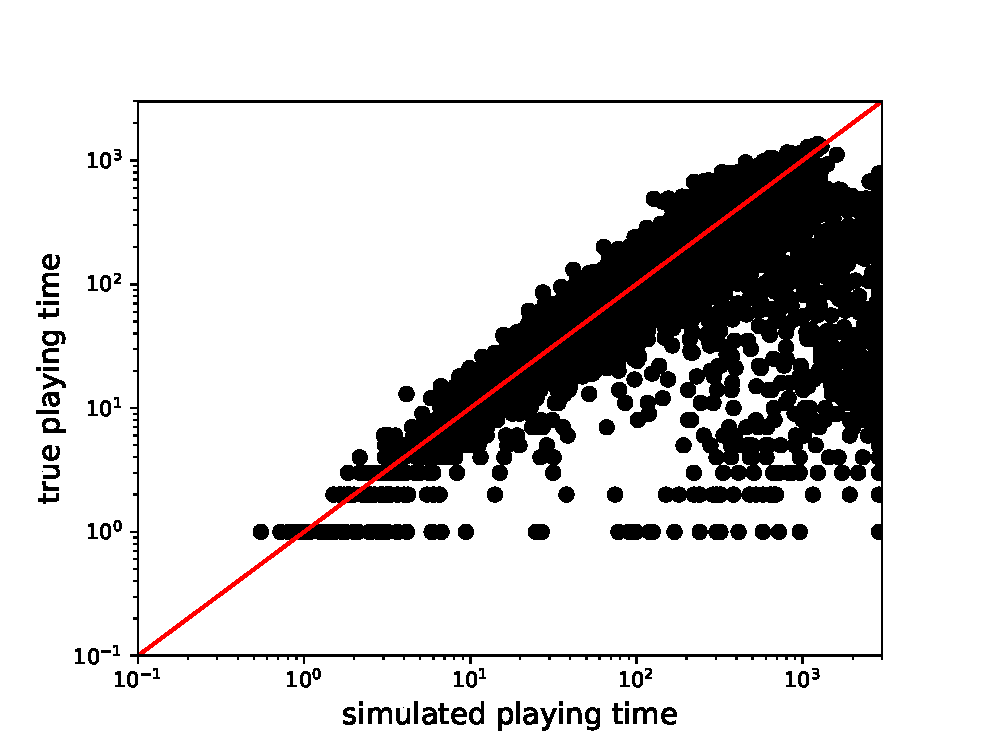
\includegraphics[width=3.5in]{plots/results/pergame_allteams_naive.eps}
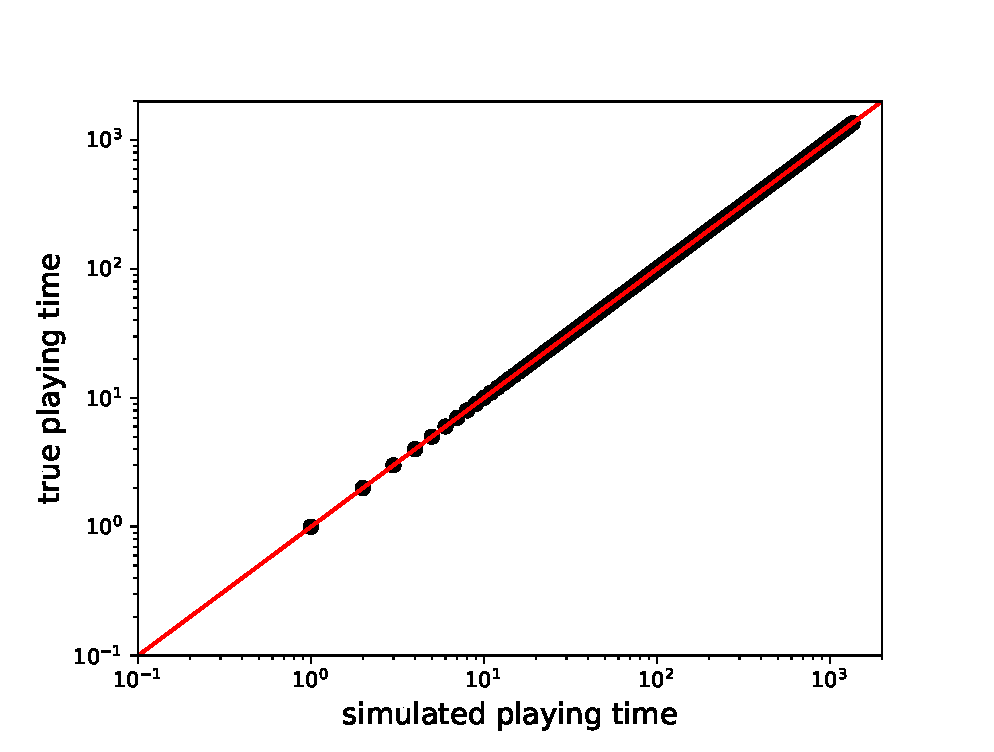
\includegraphics[width=3.5in]{plots/results/pergame_allteams.eps}
\caption{We plot simulated versus true (training set) playing times for naive (left) and fixed (right) CTMC models.   Each point on each plot corresponds to one 5-person unit for one team.  We see that the fixed model features practically zero training error, dramatically reducing the training error from the naive model.}
\label{fig:fixed_all}
\end{figure*}

\begin{figure*}[tbh]
\centering
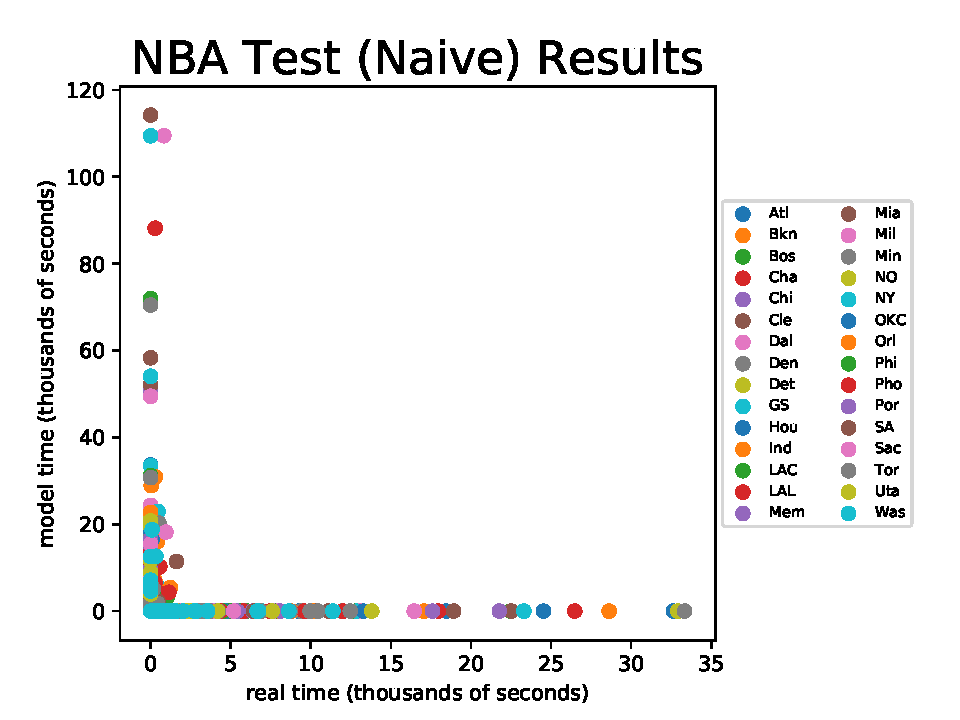
\includegraphics[width=.45\textwidth]{NBA4060_colorplots/Naive_40games_test_new.pdf}
\includegraphics[width=.45\textwidth]{NBA4060_colorplots/fixed_40games_test_new.pdf}
\caption{We plot naive (left) and fixed (right) CTMC test results using 40-game training sets.  The fixed model decreases RMSE error by $\approx 60.4\%$.  For further details, see Section \ref{sect:nbadata}.}
\label{fig:naivefixed40}
\end{figure*}

\begin{figure*}[tbh]
\center
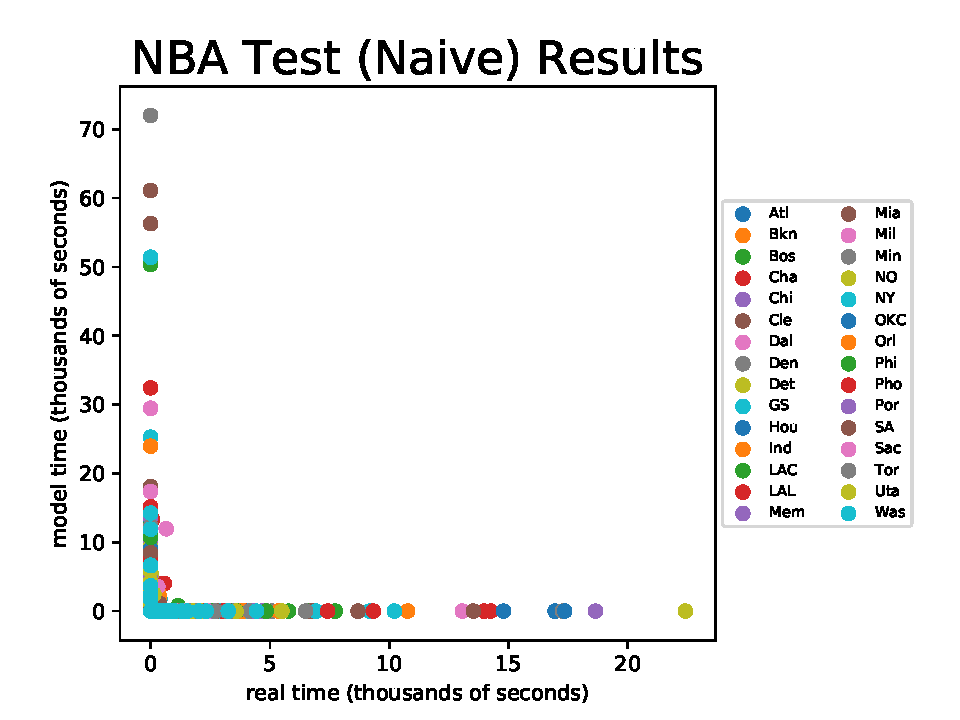
\includegraphics[width=.45\textwidth]{NBA4060_colorplots/Naive_60games_test_new.pdf}
\includegraphics[width=.45\textwidth]{NBA4060_colorplots/fixed_60games_test_new.pdf}
\caption{We plot naive (left) and fixed (right) CTMC test results using 60-game training sets.  The fixed model decreases RMSE error by $\approx 61.9\%$.  For further details, see Section \ref{sect:nbadata}.}
\label{fig:naivefixed60}
\end{figure*}

\begin{table}[tbh]
\centering
\begin{tabular}{lrrr|rrr}
\toprule
{} &  \textbf{Dim} & \textbf{NNZ} & \textbf{CV}  & \textbf{Dim} & \textbf{NNZ} & \textbf{CV} \\
\midrule
\textbf{Team} & &            &            &        &            &           \\
Atl  &    72092 &        240 &  2.167e-18 & 112560 &        274 &  4.445e-17 \\
Bkn  &    67340 &        164 &  1.484e-18 & 105950 &        272 &  4.888e-18 \\
Bos  &    90902 &        237 &  8.345e-19 & 114582 &        277 &  5.117e-18 \\
Cha  &    35532 &        185 &  1.775e-18 & 68382 &        263 &  2.957e-18 \\
Chi  &    54522 &        223 &  1.842e-18 & 151710 &        286 &  1.045e-17 \\
Cle  &    72630 &        243 &  3.305e-18 & 119370 &        275 &  4.916e-18 \\
Dal  &   110556 &        208 &  1.935e-18 & 213906 &        364 &  3.374e-18 \\
Den  &    69432 &        144 &  8.410e-19 & 144020 &        344 &  2.740e-18 \\
Det  &    13806 &        114 &  2.252e-18 & 35910 &        178 &  1.107e-18 \\
GS   &    70490 &        170 &  2.479e-18 & 120756 &        286 &  8.207e-18 \\
Hou  &    73170 &        263 &  2.690e-18 & 141000 &       2040 &  1.440e-17 \\
Ind  &    58806 &        171 &  2.730e-18 & 118680 &        280 &  3.404e-17 \\
LAC  &    55932 &        156 &  3.320e-18 & 97032 &        258 &  4.264e-18 \\
LAL  &    43056 &        132 &  2.267e-18 & 68382 &        216 &  2.339e-18 \\
Mem  &    59292 &        238 &  2.149e-18 & 181902 &        302 &  4.993e-18 \\
Mia  &    63252 &       1256 &  6.223e-17 & 114582 &       1866 &  6.285e-17 \\
Mil  &    73170 &       1241 &  2.534e-17 & 104652 &        237 &  3.334e-18 \\
Min  &    57360 &        202 &  2.542e-18 & 93942 &        235 &  3.524e-18 \\
NO   &    93942 &        193 &  2.229e-18 & 172640 &       2373 &  5.705e-17 \\
NY   &    56882 &        183 &  3.909e-18 & 99540 &        267 &  4.578e-18 \\
OKC  &    48180 &        190 &  1.604e-18 & 90300 &        234 &  1.641e-18 \\
Orl  &    57840 &        235 &  1.326e-18 & 134322 &        306 &  8.248e-18 \\
Phi  &   175980 &        280 &  9.187e-18 & 270920 &        389 &  4.804e-18 \\
Pho  &    93330 &        171 &  2.320e-18 & 234740 &        328 &  3.836e-18 \\
Por  &    34040 &       1046 &  7.235e-17 & 45582 &        236 &  1.085e-18 \\
SA   &    69432 &        243 &  5.111e-18 & 141000 &        316 &  1.709e-17 \\
Sac  &    66306 &        243 &  1.382e-18 & 102720 &        286 &  4.837e-18 \\
Tor  &    30102 &        165 &  4.034e-18 & 46010 &        204 &  3.328e-18 \\
Uta  &   113232 &        288 &  1.172e-17 & 199362 &        384 &  8.124e-18 \\
Was  &    87912 &        259 &  2.558e-18 & 146306 &        317 &  4.125e-18 \\
\bottomrule
\end{tabular}
\caption{ For each team, we compute fixed CTMC models using training sets of either the first 40 (left of bar) or 60 (right of bar) non-overtime, regular season games.  For each fixed model, we report Dim, the dimension of $\varepsilon$, equal to $M(M-1)$ where $M$ is the number of states or unique 5-person units in that team's training set.  We report NNZ, the number of nonzero entries in the computed $\varepsilon$---the small values of NNZ relative to Dim show that the computed solutions are highly sparse.  Finally, we record CV, the maximum constraint violation reported by the optimizer---all values are close to zero.}
\label{tab:sparse40}
\end{table}

\subsection{Biomedical data}
Holson and preproglucacon are discrete-time data sets from the R package \verb+markovchain+ \cite{markovchain}. The Holson data set contains life history trajectories for 1000 unique patients, each measured at 11 points in time.  The measurement at each time has value 1, 2, or 3.  We split the data into training and test sets of size 500 each.  We fit a 3-state DTMC to this data and compare the performance of naive and fixed models.

Preproglucacon data is the DNA sequence for the gene that encodes the protein preproglucacon. This data consists of 1572 observations with bases A, T, C, G coded numerically as 1, 4, 2, 3.  We split this data into a training set of size 500 and a test set of size 1072.  Using this data, we fit a 4-state DTMC and compare the performance of naive and fixed models. 

For the sake of comparison, we also fit a hidden Markov model (HMM) to both data sets.  The HMM is much more sophisticated than the DTMC and requires much more computational effort to train \cite{Fraser2008}.  When we trained HMM models, we explored hyperparameters such as the number of internal states and the random initialization of the model.  We report results for the best (smallest long-term test error) hyperparameter choices we were able to find.

Tables \ref{tab:holson} and \ref{tab:dna} show long-term training and test errors for naive DTMC, fixed DTMC, and HMM models.  The fixed DTMC models feature greatly reduced test set errors as compared to the naive DTMC models.  Note also that for the Holson data set, the long-term test errors for the fixed DTMC and HMM models are comparable.  For the preproglucacon data, the HMM's long-term test error is about 4 times less than that of the fixed DTMC.

While the HMM is able to achieve better test set results in some cases, we show in Table \ref{tab:trainingtimes} that this achievement comes at great computational expense.  We require about 50 times less computational time to produce the fixed DTMC compared to the HMM.  This includes time spent by the linear programming solver.

\begin{table}[tbh]
\centering
\begin{tabular}{lccc}
{\bf Holson} & &\\
\toprule
1-norm Error &     Naive &         Fixed  & HMM\\
\midrule
Long-term Training &  0.160545 & 1.665335e-16 & 0.000835\\
Long-term Test     &  0.235091 &  7.454545e-02 & 0.075380\\
\bottomrule
\end{tabular}
\caption{Long-term errors with training size 500 on Holson data.}
\label{tab:holson}
\end{table}

\begin{table}[tbh]
\centering
\begin{tabular}{lccc}
{\bf Preproglucacon} & &\\
\toprule
1-norm Error &     Naive &         Fixed & HMM\\
\midrule
Long-term Training &  0.003426 &  1.942890e-16 & 0.000509\\
Long-term Test     &  0.113921 &  1.154179e-01 & 0.036629\\
\bottomrule
\end{tabular}
\caption{Long-term errors with training size 500 on preproglucacon data.}
\label{tab:dna}
\end{table}

\begin{table}[tbh]
\centering
\begin{tabular}{lrr}
{\bf Training Time (seconds)} & & \\
\toprule
          Data &  Our models &   HMM \\
\midrule
        Holson &       0.71 &  54.68 \\
Preproglucacon &       0.05 &  28.40 \\
\bottomrule
\end{tabular}
\caption{Training time comparison between our models and best-case HMM models on Holson and preproglucacon data sets}
\label{tab:trainingtimes}
\end{table}

\section{Conclusion}
\label{sect:conclusion}
Both CTMC and DTMC models containing absorbing states do not capture well the observed fraction of time spent in each state.  We remove absorbing states by finding a sparse perturbation to the transition (or transition rate) matrix such that the new matrix achieves a desired equilibrium distribution. We formulated this problem as a linear programming problem.  Through extensive tests with simulated and real data, we have shown that our method improves long-term predictions without sacrificing much short-term accuracy.  Furthermore, our method requires far less time to train than HMM methods.

\section*{Acknowledgments}
H. S. Bhat gratefully acknowledges support from the National Science Foundation (DMS-1723272).  Both H. S. Bhat and L.-H. Huang gratefully acknowledge computational time on the MERCED cluster; MERCED is supported by the National Science Foundation (ACI-1429783).  This work began during the Summer of 2017 when H. S. Bhat and L-H. Huang visited the Department of Applied Mathematics at the University of Washington (Seattle)---we thank the Department for providing office space and an intellectually stimulating environment.

\section*{Appendix}
Here we derive MLEs for DTMC and CTMC models.

\subsection{DTMC}
\label{sect:dtmcmle}
Consider data consisting of a state time series $\{s_0, s_1, s_2, \ldots, s_N\}$.  Define $p_{i,j}$ to be the probability of transitioning from state $i$ to state $j$, i.e., $P(j | i)$.  Then the likelihood function is:
\begin{equation*}
L = p_{s_0, s_1} p_{s_1, s_2} \cdots p_{s_{N-1}, s_N} = \prod_{i, j} p_{i,j}^{N(i,j)}
\end{equation*}
where $N(i,j)$ is the number of times that the pattern $(i,j)$ occurs in the state time series.  Note that $p_{i,i} = 1 - \sum_{j \neq i} p_{i,j}$.  Therefore,
$$
L = \prod_{i, j : i \neq j} p_{i,j}^{N(i,j)} \prod_{i} \left(1 - \sum_{j \neq i} p_{i,j} \right)^{N(i,i)}.
$$
Fix states $i', j'$ and maximize the log likelihood function over the parameter $p_{i',j'}$:
$$
\frac{\partial \log L}{\partial p_{i',j'}} = \frac{N(i',j')}{p_{i',j'}} - \frac{N(i',i')}{1 - \sum_{j \neq i'} p_{i',j}} = 0.
$$
Suppose there are $M-1$ states in total.  Then for fixed $i'$, the above equation gives us $M-1$ equations in $M-1$ unknowns.  Let $\vec{1}$ denote the $(M-1) \times 1$ vector of all ones.  Then the $M-1$ equations can be summarized by the matrix-vector equation
$$
\left( N(i',i') I  + \vec{N} \vec{1}^T \right) \vec{p} = \vec{N}.
$$
where $\vec{N}$ is the $(M-1) \times 1$ vector
$$
\vec{N} = (N(i',1),\ldots,N(i',i'-1),N(i',i'+1),\ldots,N(i',M))
$$
and $\vec{p}$ is the $(M-1) \times 1$ vector
$$
\vec{p} = (p_{i',1},\ldots,p_{i',i'-1},p_{i',i'+1},\ldots,p_{i',M}).
$$
Note that $\vec{N} \vec{1}^T$ is a rank-1 matrix; the matrix multiplying $\vec{p}$ is therefore a rank-1 perturbation of a multiple of the identity.
We can then solve for $\vec{p}$ using the Sherman-Morrison-Woodbury matrix inversion formula:
\begin{multline*}
\left( N(i',i') I  + \vec{N} \vec{1}^T \right)^{-1} = \frac{1}{N(i',i')} I \\
- \frac{1}{N(i',i')} I \vec{N} \left( 1 + \frac{\vec{1}^T \vec{N}}{N(i',i')} \right)^{-1} \vec{1}^T \frac{1}{N(i',i')} I
\end{multline*}
Hence $\vec{p} = \vec{N} / {\sum_{j=1}^{M} N(i',j)}$.  Since $i'$ and $j'$ were arbitrary, we see that the MLE for the $(i,j)$-th entry of the transition matrix is $\widehat{p}_{i,j} = {N(i,j)}/{\sum_{k=1}^{M} N(i,k)}$.  In words, this is the number of times we observe the pattern $(i,j)$ divided by the total number of times we observe any of the patterns $(i,1), (i,2), \ldots, (i,M)$.  We have derived this formula for $i \neq j$.  Because $\widehat{p}_{i,i} = 1 - \sum_{j \neq i} \widehat{p}_{i,j}$, it is valid for $i=j$ as well.

\subsection{CTMC}
\label{sect:ctmcmle}
Consider data consisting of times $\{0=t_0, t_1, t_2, \ldots,t_N\}$ and state time series $\{s_0,s_1,s_2,\ldots, s_N \}$. Define $\alpha(x,y)$ as the rate that state $x$ jumps to state $y$.  Then the transition rate out of state $x$ is $\alpha(x) = \sum_{y \neq x} \alpha(x,y)$.  For $i = 0, \ldots, N-1$, define $T_i = t_{i+1} - t_i$.  Then the likelihood function is \cite{Guttorp}:
\begin{align*}
L &= \alpha(s_0) e^{-\alpha(s_0) T_0} \frac{\alpha(s_0,s_1)}{\alpha(s_0)} \ \alpha(s_1) e^{-\alpha(s_1) T_1} \frac{\alpha(s_1,s_2)}{\alpha(s_1)} \ \cdots \\
& =  e^{-\alpha(s_0) T_0} \alpha(s_0,s_1) \ e^{-\alpha(s_1) T_1} \alpha(s_1,s_2) \ \cdots \\
& = e^{-\sum_x \alpha(x) W(x)} \prod_{x, y: x\neq y} \alpha(x,y)^{N(x,y)},
\end{align*}
where $W(x) = \sum_{i=0}^{N-1} T_i \cdot \textbf{I}\left(s_i = x\right)$ and
$N(x,y) = \sum_{i=0}^{N-1} \textbf{I}(s_i= x, s_{i+1}=y)$.  In words, $W(x)$ is the total time spent in state $x$, and $N(x,y)$ is the total number of times that the pattern $(x,y)$ is observed.  Then
$$
\log L  = \sum_{x,y: x\neq y}[ -W(x) \alpha(x,y)+N(x,y)\log \alpha(x,y)].
$$
Fix states $x',y'$ and maximize the log likelihood function over the parameter $\alpha(x',y')$:
$$
\frac{\partial \log L}{\partial \alpha(x',y')}  = -W(x') + \frac{N(x',y')}{\alpha(x',y')}= 0.
$$
We obtain the MLE $\widehat{\alpha}(x',y') =  N(x',y') / {W(x')}$.
This holds for all $x' \neq y'$.  Hence the MLE for the $(x,y)$ entry of the transition rate matrix is the total number of transitions from state $x$ to state $y$, divided by the total time spent in state $x$.


\bibliographystyle{elsarticle-num}
\bibliography{mcopaper}

\end{document}


